% SDM Array Model — Equations and Calculations Reference
% Source: main/calculations/models/sdm_array_model.py
% Use this document to verify and track upgradations to the Single Diode Model Array.

\documentclass[11pt,a4paper]{article}
\usepackage[utf8]{inputenc}
\usepackage[T1]{fontenc}
\usepackage{amsmath,amssymb,amsthm}
\usepackage{geometry}
\usepackage{booktabs}
\usepackage{hyperref}
\usepackage{xcolor}
\usepackage{tikz}
\usetikzlibrary{shapes.geometric, arrows.meta, positioning, calc, fit}

\geometry{margin=1in}
\title{SDM Array Model\\Equations \& Calculations}
\author{Reference for \texttt{sdm\_array\_model.py}}
\date{}

\begin{document}
\maketitle
\tableofcontents
\newpage

%==============================================================================
\section{Overview}
%==============================================================================

The Single Diode Model (SDM) Array implementation:
\begin{enumerate}
  \item Fits SDM parameters \((I_{\mathrm{ph}}, I_0, R_s, R_{\mathrm{sh}}, n)\) from module datasheet (STC) once.
  \item Reuses those fitted parameters for all subsequent power calculations.
  \item Uses IV curve solving (Newton) and MPP finding (golden-section / bisection).
\end{enumerate}

\subsection{Physical Constants}

\begin{equation}
  k = 1.380649\times10^{-23}\;\mathrm{J/K} \qquad
  q = 1.602176634\times10^{-19}\;\mathrm{C}
\end{equation}

\subsection{Datasheet \& Array Structures}

\textbf{Module datasheet (STC):}
\begin{itemize}
  \item \(I_{\mathrm{sc}}\) — short-circuit current (A), \(V_{\mathrm{oc}}\) — open-circuit voltage (V)
  \item \(I_{\mathrm{mp}}, V_{\mathrm{mp}}\) — current and voltage at MPP (A, V)
  \item \(N_s\) — series cells per module
  \item \(E_g\) — bandgap (eV), Si \(\approx 1.12\;\mathrm{eV}\)
  \item \(\alpha_I\) — \(I_{\mathrm{sc}}\) temperature coefficient (A/°C)
  \item \(\beta_V\) — \(V_{\mathrm{oc}}\) temperature coefficient (fraction per °C)
\end{itemize}

\textbf{Array configuration:}
\begin{itemize}
  \item \(N_{\mathrm{ser}}\) — modules in series per string
  \item \(N_{\mathrm{par}}\) — strings in parallel
  \item \(\mathrm{NOCT}\) — Nominal Operating Cell Temperature (°C)
\end{itemize}

%==============================================================================
\section{DC Derating}
%==============================================================================

Loss fractions (each in \([0,1]\)): soiling, mismatch, dc\_ohmic, degradation, availability, others.

\begin{equation}
  \text{total\_loss} = 1 - \prod_{j} (1 - L_j)
\end{equation}

\begin{equation}
  \boxed{
  \eta_{\mathrm{dc}} = 1 - \text{total\_loss}
  }
\end{equation}

So \(P_{\mathrm{dc}} = P_{\mathrm{dc,raw}} \cdot \eta_{\mathrm{dc}}\).

%==============================================================================
\section{Thermal Model (Faiman)}
%==============================================================================

Cell temperature from plane-of-array irradiance \(G\), ambient temperature \(T_{\mathrm{amb}}\) (°C), and wind speed \(v_{\mathrm{wind}}\) (m/s):

\begin{equation}
  U_{\mathrm{sum}} = \frac{800}{\max(\mathrm{NOCT} - 20,\; 10^{-6})}
  \quad \text{(W/m}^2\text{-K)}
\end{equation}

\begin{equation}
  U_0 = 0.8\, U_{\mathrm{sum}}, \qquad U_1 = 0.2\, U_{\mathrm{sum}}
\end{equation}

\begin{equation}
  \boxed{
  T_{\mathrm{cell}} = T_{\mathrm{amb}} + \frac{G}{U_0 + U_1\cdot\max(v_{\mathrm{wind}}, 0)}
  }
\end{equation}

%==============================================================================
\section{SDM Primitives}
%==============================================================================

\subsection{Thermal Voltage (module)}

\begin{equation}
  \boxed{
  V_t = \frac{k\,T}{q}\,N_s
  }
\end{equation}
with \(T\) in Kelvin.

\subsection{Single-Diode IV Equation}

The output current \(I\) at voltage \(V\) is given implicitly by:
\begin{equation}
  \boxed{
  I = I_{\mathrm{ph}} - I_0\left(\exp\frac{V + I R_s}{n\,V_t} - 1\right) - \frac{V + I R_s}{R_{\mathrm{sh}}}
  }
\end{equation}

Newton iteration: define
\begin{align}
  e_a &= \frac{V + I R_s}{n\,V_t}, \quad e_a \in [-60,\,60] \\
  e &= \exp(e_a)
\end{align}

Residual and derivative with respect to \(I\):
\begin{align}
  f(I) &= I - I_{\mathrm{ph}} + I_0(e - 1) + \frac{V + I R_s}{R_{\mathrm{sh}}} \\
  \frac{\partial f}{\partial I} &= 1 + I_0\,e\,\frac{R_s}{n\,V_t} + \frac{R_s}{R_{\mathrm{sh}}}
\end{align}

Update:
\begin{equation}
  \Delta I = \frac{f}{\max(\partial f/\partial I,\; 10^{-16})}, \qquad
  I_{\mathrm{new}} = I - \operatorname{clip}(\Delta I,\; -2,\; 2)
\end{equation}

Iterate until \(|I_{\mathrm{new}} - I| < 10^{-10}\); then \(I \leftarrow \max(I_{\mathrm{new}},\; 0)\).

\subsection{Derivative \(\mathrm{d}I/\mathrm{d}V\)}

\begin{equation}
  A = \frac{I_0\,e}{n\,V_t} + \frac{1}{R_{\mathrm{sh}}}, \qquad
  B = 1 + R_s\,A
\end{equation}

\begin{equation}
  \boxed{
  \frac{\mathrm{d}I}{\mathrm{d}V} = -\frac{A}{\max(B,\; 10^{-16})}
  }
\end{equation}

At MPP: \(I_{\mathrm{mp}} + V_{\mathrm{mp}}\,\frac{\mathrm{d}I}{\mathrm{d}V}\big|_{V_{\mathrm{mp}}} = 0\).

%==============================================================================
\section{Fit SDM from STC}
%==============================================================================

Given module datasheet at \(T_{\mathrm{cell}} = 25°\mathrm{C}\): fit \(\theta = (I_{\mathrm{ph}},\; \log_{10}I_0,\; R_s,\; R_{\mathrm{sh}},\; n)\).

Bounds:
\begin{align}
  I_{\mathrm{ph}} &\in [0.98\,I_{\mathrm{sc}},\; 1.02\,I_{\mathrm{sc}}] \\
  \log_{10}I_0 &\in [-40,\; -2] \\
  R_s &\in [10^{-4},\; 2], \quad R_{\mathrm{sh}} \in [10,\; 5000], \quad n \in [1,\; 2.5]
\end{align}

Residuals (to be driven to zero by least-squares):
\begin{align}
  r_1 &= I(V{=}0) - I_{\mathrm{sc}} \\
  r_2 &= I(V{=}V_{\mathrm{oc}}) - 0 \\
  r_3 &= I(V{=}V_{\mathrm{mp}}) - I_{\mathrm{mp}} \\
  r_4 &= I_{\mathrm{mp}} + V_{\mathrm{mp}}\,\frac{\mathrm{d}I}{\mathrm{d}V}\bigg|_{V_{\mathrm{mp}}} \quad \text{(MPP slope)} \\
  r_5 &= I_{\mathrm{ph}} - I_{\mathrm{sc}} \quad \text{(soft tie)}
\end{align}

Multiple seeds over \(R_s \in \{0.1,\,0.3,\,0.6\}\), \(R_{\mathrm{sh}} \in \{200,\,500,\,1000\}\), \(n \in \{1.15,\,1.3,\,1.5\}\); initial \(I_0\) guess:
\begin{equation}
  I_0^{\mathrm{guess}} = \frac{I_{\mathrm{sc}}}{\exp(V_{\mathrm{oc}}/(n\,V_t)) - 1 + 10^{-30}}
\end{equation}

Best solution (lowest cost) is kept; returns \(I_{\mathrm{ph}}, I_0, R_s, R_{\mathrm{sh}}, n, V_{t,\mathrm{ref}}, T_{\mathrm{ref}}\).

%==============================================================================
\section{Voc and MPP Solvers}
%==============================================================================

\subsection{Open-Circuit Voltage (bisection)}

Initial guess (ideal diode):
\begin{equation}
  V_{\mathrm{oc}}^{\mathrm{guess}} = n\,V_t\,\ln\left(1 + \frac{I_{\mathrm{ph}}}{\max(I_0,\,10^{-30})}\right)
\end{equation}

Bracket: \([0,\; V_{\mathrm{oc}}^{\mathrm{guess}}]\); expand upper bound until \(I(V_{\mathrm{hi}}) \le 0\). Bisect until \(|\mathrm{hi} - \mathrm{lo}| < 10^{-7}\); \(V_{\mathrm{oc}} = (\mathrm{lo}+\mathrm{hi})/2\).

\subsection{MPP: direct Newton on \(g(V)=0\) (preferred)}

At MPP, \(\mathrm{d}P/\mathrm{d}V = I + V\,\mathrm{d}I/\mathrm{d}V = 0\). With \(f(V,I)=0\) we have \(\mathrm{d}I/\mathrm{d}V = -f_V/f_I\). So the MPP condition is
\begin{equation}
  g(V) = I - V\,\frac{f_V}{f_I} = 0.
\end{equation}
Algorithm: Newton on \(g(V)\). At each outer iteration: (1)~solve \(f(V,I)=0\) for \(I\) (one inner Newton, \texttt{iv\_current}); (2)~compute \(f_V\), \(f_I\), and second derivatives \(f_{VV}\), \(f_{VI}\), \(f_{II}\); (3)~\(g' = -2 f_V/f_I - V\,(f_V/f_I)'\) with \((f_V/f_I)' = (f_{VV}f_I^2 - 2 f_V f_{VI} f_I + f_V^2 f_{II})/f_I^3\); (4)~\(V \leftarrow V - g/g'\). Typically converges in 2--4 outer iterations. No golden-section or voltage sweep. If Newton does not converge, the code falls back to golden-section (\texttt{mpp\_golden}).

\subsection{MPP fallback: golden-section on \(P(V) = V\,I(V)\))}

\begin{equation}
  \varphi = \frac{\sqrt{5}-1}{2}, \qquad
  \text{bracket: } [a,b] = [0,\; 0.999\,V_{\mathrm{oc}}]
\end{equation}

Golden-section search on \(P(V)\) until \(|b-a| < 10^{-6}\); then
\begin{equation}
  V_{\mathrm{mp}} = \frac{a+b}{2}, \qquad
  I_{\mathrm{mp}} = I(V_{\mathrm{mp}}), \qquad
  P_{\mathrm{mp}} = V_{\mathrm{mp}}\,I_{\mathrm{mp}}
\end{equation}
Used only if \texttt{mpp\_newton} fails.

%==============================================================================
\section{Real-Time Power Estimation}
%==============================================================================

Inputs: \(G_{\mathrm{poa}}\), \(T_{\mathrm{amb}}\), \(v_{\mathrm{wind}}\), module datasheet, array config, derates, fitted params.

\subsection{Cell temperature}
\begin{equation}
  T_{\mathrm{cell}} = \text{Faiman}(G_{\mathrm{poa}}, T_{\mathrm{amb}}, v_{\mathrm{wind}}, \mathrm{NOCT})
\end{equation}
\(T = T_{\mathrm{cell}} + 273.15\), \(T_{\mathrm{ref}} = T_{\mathrm{ref},C} + 273.15\).

\subsection{Thermal voltage at operating \(T\)}
\begin{equation}
  V_t = \frac{k\,T}{q}\,N_s
\end{equation}

\subsection{Saturation current at \(T\)}
\begin{equation}
  \boxed{
  I_0(T) = I_{0,\mathrm{ref}}\,\left(\frac{T}{T_{\mathrm{ref}}}\right)^3\,
  \exp\left(\frac{q\,E_g}{n\,k}\left(\frac{1}{T_{\mathrm{ref}}} - \frac{1}{T}\right)\right)
  }
\end{equation}

\subsection{Photocurrent at \((G,T)\)}
\begin{equation}
  \boxed{
  I_{\mathrm{ph}} = \left(I_{\mathrm{sc}} + \alpha_I\,(T_{\mathrm{cell}} - 25)\right)\,\frac{G_{\mathrm{poa}}}{1000}
  }
\end{equation}

\subsection{Module MPP}
\begin{equation}
  (V_{\mathrm{mp,mod}},\; I_{\mathrm{mp,mod}},\; P_{\mathrm{mp,mod}}) = \text{mpp\_golden}(I_{\mathrm{ph}}, I_0, R_s, R_{\mathrm{sh}}, n, V_t)
\end{equation}

\subsection{String and array scaling}
\begin{align}
  V_{\mathrm{mp,str}} &= N_{\mathrm{ser}}\,V_{\mathrm{mp,mod}}, \quad
  I_{\mathrm{mp,str}} = I_{\mathrm{mp,mod}}, \quad
  P_{\mathrm{mp,str}} = V_{\mathrm{mp,str}}\,I_{\mathrm{mp,str}} \\
  V_{\mathrm{mp,arr}} &= V_{\mathrm{mp,str}}, \quad
  I_{\mathrm{mp,arr}} = N_{\mathrm{par}}\,I_{\mathrm{mp,str}} \\
  P_{\mathrm{dc,raw}} &= V_{\mathrm{mp,arr}}\,I_{\mathrm{mp,arr}}
\end{align}

\subsection{DC derating}
\begin{equation}
  \boxed{
  P_{\mathrm{dc}} = P_{\mathrm{dc,raw}}\,\eta_{\mathrm{dc}}
  }
\end{equation}

%==============================================================================
\section{Degradation (installation age)}
%==============================================================================

\begin{equation}
  \text{age\_years} = \frac{\text{(today} - \text{installation\_date).days}}{365.25}
\end{equation}

If \texttt{measured\_degradation\_rate} is set:
\begin{equation}
  \text{total\_degradation\_pct} = \text{measured\_degradation\_rate} \times \text{age\_years}
\end{equation}

Else (warranty-based):
\begin{equation}
  \text{total\_degradation\_pct} =
  \begin{cases}
    \text{estimated\_degradation\_year1} & \text{if } \text{age\_years} \le 1 \\
    \text{year1\_deg} + (\text{age\_years} - 1)\,\text{annual\_deg} & \text{otherwise}
  \end{cases}
\end{equation}

Degradation is applied as one of the loss terms in the derate factor \(\eta_{\mathrm{dc}}\).

%==============================================================================
\section{Where MPP/Vmpp time is spent (code locations)}
%==============================================================================

The ``MPP / Vmpp calculation'' timing (\texttt{estimate\_power\_vmpp\_ms}) is the time for the whole \texttt{estimate\_power()} call. Almost all of that time is inside \texttt{mpp\_golden()}, which finds the maximum power point by (1)~finding \(V_{\mathrm{oc}}\) with bisection and (2)~maximizing \(P(V)=V\,I(V)\) with golden-section search. Both steps call \texttt{iv\_current()} many times, and each \texttt{iv\_current()} can run up to 60 Newton iterations. That is why this step dominates.

\subsection{Code locations (file: \texttt{sdm\_array\_model.py})}

\begin{itemize}
  \item \textbf{Timing wrapped around:} \texttt{calculate\_expected\_power()} calls \texttt{estimate\_power()} and records the elapsed time as \texttt{estimate\_power\_vmpp\_ms} (lines 698--708).
  \item \textbf{Entry:} \texttt{estimate\_power()} (lines 245--283). Steps 1--3 (Faiman, \(V_t\), \(I_0\), \(I_{\mathrm{ph}}\)) are cheap. Step 4 is the expensive one.
  \item \textbf{Expensive step:} \texttt{mpp\_golden(Iph, I0, Rs, Rsh, n, Vt)} (line 263) \(\rightarrow\) defined at lines 205--239.
  \item \textbf{Inside \texttt{mpp\_golden}:}
  \begin{itemize}
    \item \texttt{voc\_bisect(...)} (line 212) \(\rightarrow\) defined at lines 174--203. Up to 40 bracket expansions + 80 bisection iterations; each iteration calls \texttt{I\_of\_V(V)} \(\equiv\) \texttt{iv\_current(V, ...)}.
    \item Golden-section loop: 100 iterations (lines 219--232); each iteration evaluates \texttt{P\_of\_V} once or twice, and \texttt{P\_of\_V(V)} calls \texttt{I\_of\_V(V)} \(\equiv\) \texttt{iv\_current(V, ...)}.
  \end{itemize}
  \item \textbf{Core cost:} \texttt{iv\_current(V, Iph, I0, Rs, Rsh, n, Vt)} (lines 91--106). For each voltage \(V\), Newton iteration runs up to 60 times (line 94) until \(|I_{\mathrm{new}} - I| < 10^{-10}\). Each iteration uses \(\exp(\cdot)\), so the total number of exponentials per MPP is roughly \((\text{bisection} + \text{golden})\times \text{Newton}\) \(\approx (80 + 200)\times \text{avg Newton}\).
\end{itemize}

So the 211\,ms (or similar) is almost entirely: \texttt{mpp\_golden} \(\to\) \texttt{voc\_bisect} (many \texttt{iv\_current}) + golden-section (many \texttt{iv\_current}), with each \texttt{iv\_current} doing a Newton solve.

%==============================================================================
\section{Flowcharts}
%==============================================================================

\subsection{Overall calculation flow}

\begin{center}
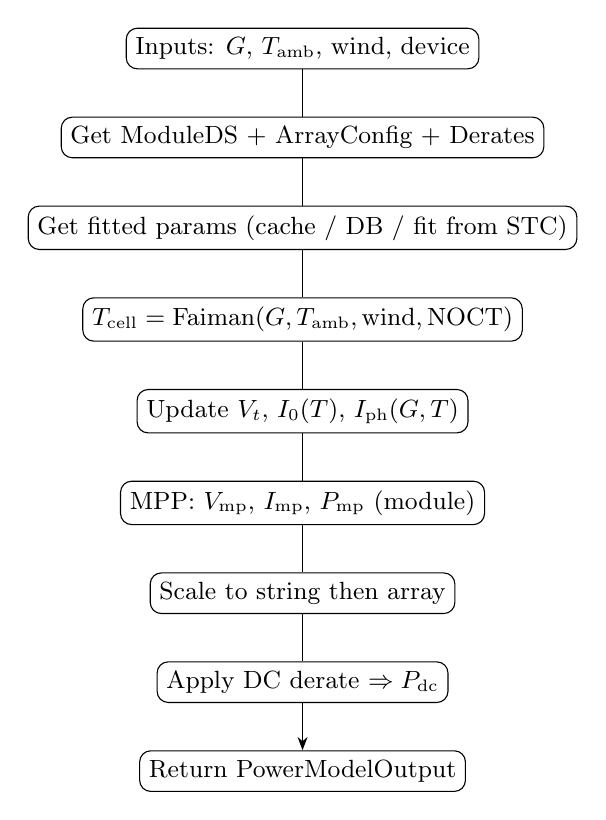
\begin{tikzpicture}[
  node distance=0.6cm and 1.2cm,
  box/.style={rectangle, draw, rounded corners, minimum width=2.2cm, minimum height=0.5cm, align=center, font=\small},
  decision/.style={diamond, draw, aspect=2, minimum width=1.4cm, align=center, font=\small},
  arrow/.style={-Stealth}
]
  \node[box] (A) {Inputs: $G$, $T_{\mathrm{amb}}$, wind, device};
  \node[box, below=of A] (B) {Get ModuleDS + ArrayConfig + Derates};
  \node[box, below=of B] (C) {Get fitted params (cache / DB / fit from STC)};
  \node[box, below=of C] (D) {$T_{\mathrm{cell}} = \mathrm{Faiman}(G, T_{\mathrm{amb}}, \mathrm{wind}, \mathrm{NOCT})$};
  \node[box, below=of D] (E) {Update $V_t$, $I_0(T)$, $I_{\mathrm{ph}}(G,T)$};
  \node[box, below=of E] (F) {MPP: $V_{\mathrm{mp}}$, $I_{\mathrm{mp}}$, $P_{\mathrm{mp}}$ (module)};
  \node[box, below=of F] (G) {Scale to string then array};
  \node[box, below=of G] (H) {Apply DC derate $\Rightarrow P_{\mathrm{dc}}$};
  \node[box, below=of H] (I) {Return PowerModelOutput};
  \draw[arrow] (A) -- (B) (B) -- (C) (C) -- (D) (D) -- (E) (E) -- (F) (F) -- (G) (G) -- (H) (H) -- (I);
\end{tikzpicture}
\end{center}

\subsection{Parameter resolution (fitted SDM params)}

\begin{center}
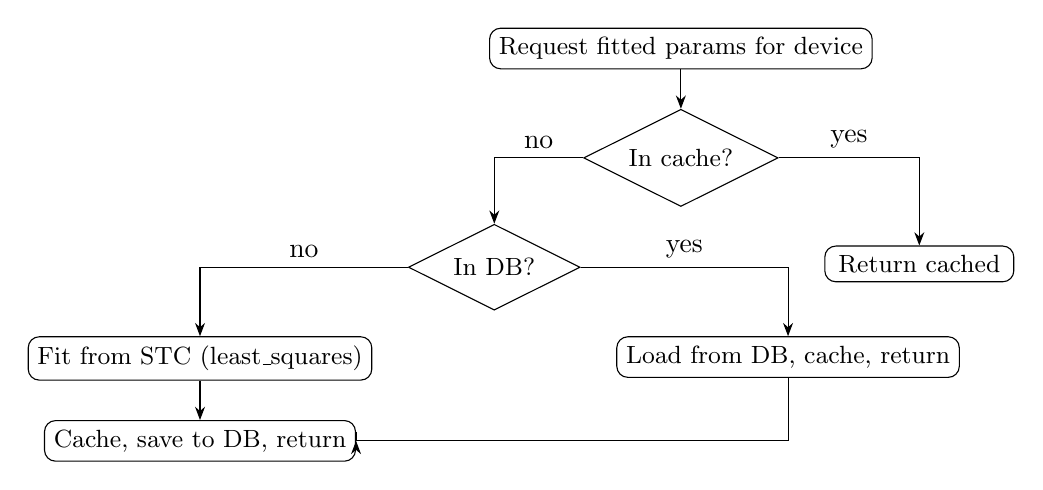
\begin{tikzpicture}[
  node distance=0.5cm and 1cm,
  box/.style={rectangle, draw, rounded corners, minimum width=2.4cm, minimum height=0.45cm, align=center, font=\small},
  decision/.style={diamond, draw, aspect=2, minimum width=1.6cm, align=center, font=\small},
  arrow/.style={-Stealth}
]
  \node[box] (A) {Request fitted params for device};
  \node[decision, below=of A] (B) {In cache?};
  \node[box, below right=0.8cm and 1.2cm of B] (C) {Return cached};
  \node[decision, below left=0.8cm and 1.2cm of B] (D) {In DB?};
  \node[box, below right=0.6cm and 1cm of D] (E) {Load from DB, cache, return};
  \node[box, below left=0.6cm and 1cm of D] (F) {Fit from STC (least\_squares)};
  \node[box, below=of F] (G) {Cache, save to DB, return};
  \draw[arrow] (A) -- (B);
  \draw[arrow] (B) -| (C) node[pos=0.25, above] {yes};
  \draw[arrow] (B) -| (D) node[pos=0.25, above] {no};
  \draw[arrow] (D) -| (E) node[pos=0.25, above] {yes};
  \draw[arrow] (D) -| (F) node[pos=0.25, above] {no};
  \draw[arrow] (F) -- (G);
  \draw[arrow] (E) |- ([xshift=0.5cm]G.east) -| (G.east);
\end{tikzpicture}
\end{center}

\subsection{IV current (Newton) and MPP}

\begin{center}
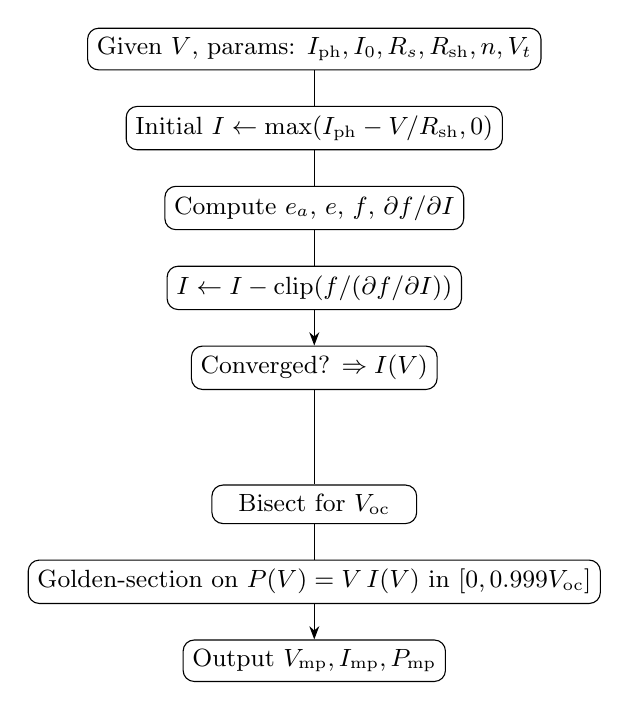
\begin{tikzpicture}[
  node distance=0.45cm and 1cm,
  box/.style={rectangle, draw, rounded corners, minimum width=2.6cm, minimum height=0.4cm, align=center, font=\small},
  arrow/.style={-Stealth}
]
  \node[box] (A) {Given $V$, params: $I_{\mathrm{ph}}, I_0, R_s, R_{\mathrm{sh}}, n, V_t$};
  \node[box, below=of A] (B) {Initial $I \leftarrow \max(I_{\mathrm{ph}} - V/R_{\mathrm{sh}}, 0)$};
  \node[box, below=of B] (C) {Compute $e_a$, $e$, $f$, $\partial f/\partial I$};
  \node[box, below=of C] (D) {$I \leftarrow I - \mathrm{clip}(f/(\partial f/\partial I))$};
  \node[box, below=of D] (E) {Converged? $\Rightarrow I(V)$};
  \node[box, below=1.2cm of E] (F) {Bisect for $V_{\mathrm{oc}}$};
  \node[box, below=of F] (G) {Golden-section on $P(V)=V\,I(V)$ in $[0, 0.999 V_{\mathrm{oc}}]$};
  \node[box, below=of G] (H) {Output $V_{\mathrm{mp}}, I_{\mathrm{mp}}, P_{\mathrm{mp}}$};
  \draw[arrow] (A) -- (B) (B) -- (C) (C) -- (D) (D) -- (E);
  \draw[arrow] (E) -- (F) (F) -- (G) (G) -- (H);
\end{tikzpicture}
\end{center}

\subsection{MPP / Vmpp calculation flow (where the time goes)}

The following flowchart shows exactly how the MPP step runs and why it costs the most. All timed work under ``estimate\_power\_vmpp\_ms'' is inside \texttt{estimate\_power()}; the dominant part is \texttt{mpp\_golden}, which uses \texttt{iv\_current} (Newton) many times.

\begin{center}
\small
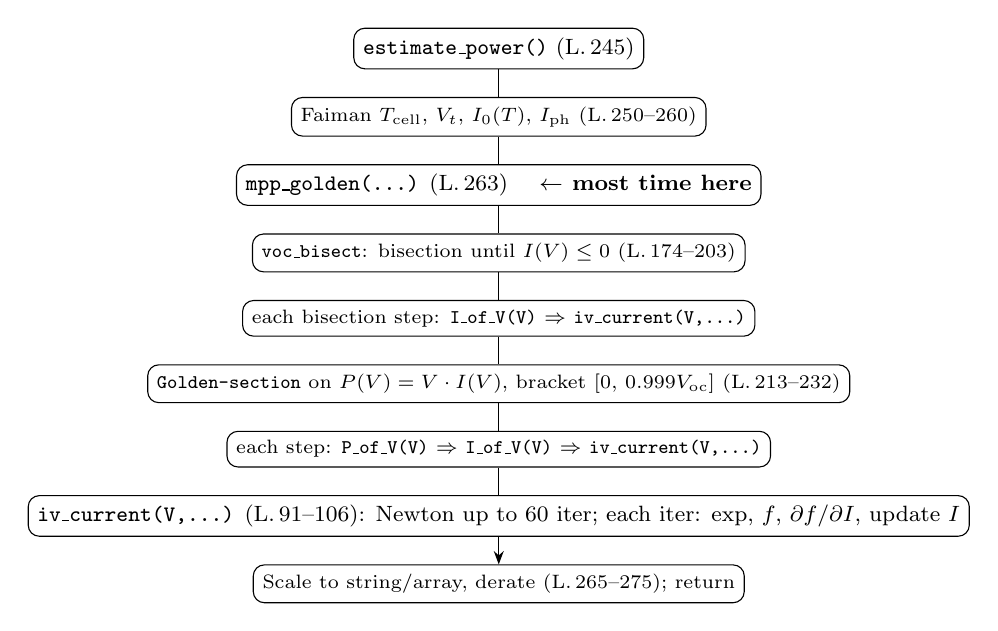
\begin{tikzpicture}[
  node distance=0.35cm and 0.9cm,
  box/.style={rectangle, draw, rounded corners, minimum height=0.4cm, align=center, font=\footnotesize},
  smallbox/.style={rectangle, draw, rounded corners, minimum height=0.35cm, align=center, font=\scriptsize},
  arrow/.style={-Stealth}
]
  \node[box] (EP) {\texttt{estimate\_power()} (L.\,245)};
  \node[smallbox, below=of EP] (Faiman) {Faiman $T_{\mathrm{cell}}$, $V_t$, $I_0(T)$, $I_{\mathrm{ph}}$ (L.\,250--260)};
  \node[box, below=of Faiman] (MPPcall) {\texttt{mpp\_golden(...)} (L.\,263) \quad \textbf{$\leftarrow$ most time here}};
  \node[smallbox, below=of MPPcall] (Voc) {\texttt{voc\_bisect}: bisection until $I(V)\le 0$ (L.\,174--203)};
  \node[smallbox, below=of Voc] (IVvoc) {each bisection step: \texttt{I\_of\_V(V)} $\Rightarrow$ \texttt{iv\_current(V,...)}};
  \node[smallbox, below=of IVvoc] (Golden) {\texttt{Golden-section} on $P(V)=V\cdot I(V)$, bracket $[0,\,0.999 V_{\mathrm{oc}}]$ (L.\,213--232)};
  \node[smallbox, below=of Golden] (IVgold) {each step: \texttt{P\_of\_V(V)} $\Rightarrow$ \texttt{I\_of\_V(V)} $\Rightarrow$ \texttt{iv\_current(V,...)}};
  \node[box, below=of IVgold] (IVcur) {\texttt{iv\_current(V,...)} (L.\,91--106): Newton up to 60 iter; each iter: $\exp$, $f$, $\partial f/\partial I$, update $I$};
  \node[smallbox, below=of IVcur] (Scale) {Scale to string/array, derate (L.\,265--275); return};
  \draw[arrow] (EP) -- (Faiman) (Faiman) -- (MPPcall) (MPPcall) -- (Voc) (Voc) -- (IVvoc) (IVvoc) -- (Golden) (Golden) -- (IVgold) (IVgold) -- (IVcur) (IVcur) -- (Scale);
\end{tikzpicture}
\end{center}

Rough count per single MPP call: voc\_bisect $\sim$ 80--120 evaluations of $I(V)$, golden-section $\sim$ 200 evaluations of $P(V)$ (each $= V\cdot I(V)$). So $\sim$ 280--320 calls to \texttt{iv\_current}, each with up to 60 Newton iterations. That explains the high ``MPP / Vmpp calculation'' time (e.g. 211\,ms).

%==============================================================================
\section{Version history (upgradations)}
%==============================================================================

Use the table below to record changes when you upgrade the model.

\begin{center}
\begin{tabular}{cll}
  \toprule
  Date & Section / Equation & Change \\
  \midrule
  (initial) & — & Document created from \texttt{sdm\_array\_model.py}. \\
  \bottomrule
\end{tabular}
\end{center}

\end{document}
